% Tipo de documento y configuración de página
\documentclass[11pt,a4paper]{article}
\usepackage[left=3.0cm, right=3.0cm, top=2.5cm, bottom=2.5cm]{geometry}

% Codificación del input e idioma
\usepackage[utf8]{inputenc}
\usepackage[spanish]{babel}
\usepackage{csquotes}
\usepackage[spanish]{datetime2}

% Texto y matemática en fuente sans serif
\usepackage{cmbright}

% Matemática
\usepackage{amsmath}
% \usepackage{amssymb}

% Unidades del SI
\usepackage{siunitx}
\sisetup{group-separator = {\text{.}}}
\DeclareSIUnit{\angstrom}{\text{\AA}}

% Figuras, tablas y código
\usepackage{graphicx}
\usepackage{float}
\usepackage{booktabs}
\usepackage{xcolor}
\usepackage{caption}
\DeclareCaptionFormat{gris}{%
  \colorbox{gray!10}{\parbox{\dimexpr\linewidth-2\fboxsep\relax}{#1#2#3}}}
\captionsetup{format=gris}
\usepackage{tikz}
\usetikzlibrary{positioning, arrows.meta, fit}
\usepackage{listings}
\lstset{
    basicstyle=\small\ttfamily,
    columns=fullflexible,
    keepspaces=true,
    frame=single,
    framesep=4pt,
    rulecolor=\color{gray!60},
    breaklines=true,
    aboveskip=0.6em,
    belowskip=0.6em}

% Bibliografía
\usepackage{hyperref}
\hypersetup{colorlinks=true, linkcolor=black, citecolor=black,
            urlcolor=blue!50!black}
\usepackage[sorting=none, url=false, doi=true, eprint=false, isbn=false,
            maxnames=10]{biblatex}
\addbibresource{referencias.bib}
\renewcommand*{\bibfont}{\small}
\setcounter{biburlnumpenalty}{9000}
\setcounter{biburllcpenalty}{9000}
\setcounter{biburlucpenalty}{9000}

% Datos del trabajo
\newcommand{\urlrepositorio}{https://github.com/santiagomosca/flujo_nt}
\newcommand{\paquete}{\texttt{flujo\_nt}}
\newcommand{\comando}{\texttt{flujo-nt}}

% Marcas de borrador: se eliminan antes de entregar
\newcommand{\pendiente}[1]{\textcolor{red}{[Pendiente: #1]}}

\title{\textbf{\Large \paquete: reescritura orientada a objetos de las
       herramientas de análisis de flujo a través de nanotubos}}
\author{}
\date{}

\begin{document}

\maketitle
\vspace{-4em} % reduzco espacio entre título y datos

% Debajo del título
\begin{flushleft}
\textbf{Trabajo final:} Herramientas Computacionales para Científicos
(UNLP -- UTN FRLP) \\
\textbf{Docentes:} Manuel Carlevaro, Ramiro Irastorza \\
\textbf{Alumno:} Santiago Mosca \\
\textbf{Repositorio:} \url{\urlrepositorio} \\
\textbf{Fecha:} \today
\end{flushleft}
\vspace{1em} % aumento espacio entre datos y texto

%/ ======================================================================
\section{Introducción}

Este trabajo se enmarca en mi tesis del Doctorado en Ingeniería, mención
Materiales, de la Universidad Tecnológica Nacional, Facultad Regional La
Plata, titulada \enquote{Flujo y transporte en medios porosos} y dirigida por
el Dr. Manuel Carlevaro. En ese contexto, y durante mi estadía como becario
doctoral de CONICET en el Instituto de Física de Líquidos y Sistemas
Biológicos (IFLySiB, UNLP--CONICET), estudié mediante simulaciones de
dinámica molecular, realizadas con LAMMPS~\cite{lammps}, el transporte de
mezclas de agua y metanol a través de nanotubos de grafeno, como modelo
simplificado del proceso de pervaporación a través de los canales de una
membrana hidrofóbica.

El sistema consiste en un nanotubo de grafeno de pared simple, de
\SI{131.25}{\angstrom} de largo y \SI{10.5}{\angstrom} o
\SI{21}{\angstrom} de diámetro, unido por sus extremos a dos láminas de
grafeno que delimitan los reservorios; el agua se modeló con el potencial
TIP4P/2005 y el metanol con OPLS/2016, en mezclas con fracción molar de
metanol de \num{0.115} y \num{0.692}. Cada simulación se desarrolla en dos
etapas. En la primera, a \SI{298}{\kelvin}, el sistema es periódico en las
tres direcciones y el tubo está alineado con el eje $x$, de modo que el
fluido a ambos lados del tubo se conecta a través de la frontera periódica y
forma un único reservorio, desde el cual la mezcla llena el tubo mientras se
insertan moléculas en las zonas donde la densidad baja, para mantener la
densidad y la composición del reservorio. En la segunda, destinada a estudiar
la pervaporación a \SI{398}{\kelvin}, las moléculas de un lado del tubo se
trasladan al otro y los extremos de la celda se cierran con láminas de
grafeno puramente repulsivas, de modo que queda un reservorio lleno, de
doble largo, otro vacío y el tubo todavía lleno de la mezcla. Esta etapa
exige cortar la periodicidad a lo largo del eje del tubo, y con ella cambia
el tratamiento de las interacciones coulombianas de largo alcance, que pasan
a calcularse sólo en las direcciones periódicas mediante una geometría de
slab: LAMMPS la implementa con la opción \texttt{kspace\_modify slab}, que
inserta vacío entre las réplicas en la dirección cortada y elimina la
interacción dipolar entre ellas, pero que sólo admite que esa dirección sea
$z$, por lo que en esta etapa el tubo debe alinearse con ese eje.

Cada simulación produce trayectorias en formato netCDF con la convención de
AMBER~\cite{amber_netcdf}, con del orden de $10^5$ partículas (\num{101112}
en el sistema que se usa como ejemplo en este trabajo) registradas en
\num{1001} cuadros por cada tramo de \SI{1}{\nano\second}, lo que da
archivos de unos \SI{6}{\giga\byte}. Para extraer de ellas el flujo de cada
especie a través del tubo, la densidad y el perfil de velocidad en función
de la distancia al eje, la densidad a lo largo del eje y la cantidad de
moléculas que alcanzan el reservorio receptor, desarrollé una biblioteca de
funciones en Python, con cálculos vectorizados con NumPy~\cite{numpy} y un
tratamiento del tubo como lo que es durante la simulación, un cilindro que
se curva, y alrededor de ella una decena de scripts, uno por análisis. Con
esas herramientas se obtuvieron los resultados publicados
en~\cite{mosca2025}, cuyo hallazgo principal es que, una vez alcanzado el
equilibrio en el reservorio receptor, la concentración de alcohol supera
ampliamente la que correspondería al equilibrio líquido-vapor sin
confinamiento, sobre todo a partir de soluciones diluidas y en tubos dos a
tres veces más anchos que el tamaño medio de las moléculas.

Ese código, sin embargo, creció sobre la marcha, a medida que el trabajo
pedía nuevos análisis, y acumuló tres limitaciones: las sucesivas versiones
de la biblioteca convivían, de modo que una misma función aparecía con
variantes entre ellas y entre los scripts que las usaban; cada script
cargaba la trayectoria completa en memoria; y los análisis suponían el tubo
alineado con el eje $x$, por lo que las trayectorias de la etapa de
pervaporación debían rotarse antes de analizarse, y esas rotaciones, al
duplicar la trayectoria en memoria, la agotaban en los sistemas más grandes.
Como buena parte del código era reutilizable, para el trabajo final de este
curso me propuse reescribirlo como un paquete de Python, \paquete, con tres
metas: un diseño orientado a objetos, como el que se promovió en el curso
tanto para Python como para C++; un desarrollo versionado, publicado en un
repositorio e instalable como paquete; y un uso de memoria independiente del
largo de la trayectoria, que aprovechara los algoritmos ya diseñados para
hacerlos todavía más eficientes y permitiera analizar las trayectorias en
cualquier orientación sin rotarlas. El fin es que la herramienta pueda
compartirse y ser reutilizada por otros integrantes del grupo de
investigación, o por quien analice simulaciones similares.

%/ ======================================================================
\section{Herramientas computacionales utilizadas}

\subsection{Lenguaje, bibliotecas y entorno de desarrollo}

El paquete está escrito en Python (3.9 o posterior) y depende sólo de NumPy, para
todo el cálculo numérico, y de netCDF4-python~\cite{netcdf4python}, para leer
las trayectorias; todas las herramientas usadas son software libre. Se evaluó
usar una biblioteca general de análisis de trayectorias como
MDAnalysis~\cite{mdanalysis}, pero se descartó: agrega dependencias, impone
sus propias unidades (picosegundos, mientras que las trayectorias registran
femtosegundos) y no resuelve los cálculos específicos del problema. Leer el
archivo netCDF directamente da control sobre qué se lee y cuándo, que es la
clave del ahorro de memoria.

El código se versiona con git y se publica en GitHub. Se empaqueta con
\texttt{pyproject.toml} y la estructura \texttt{src}, de modo que se instala
con \texttt{pip}, que además crea el comando \comando. Los tests se escriben
con pytest~\cite{pytest}, el estilo se controla con pycodestyle según
PEP~8~\cite{pep8}, y la documentación sigue la convención
numpydoc~\cite{numpydoc}, que en lugar de anotaciones de tipo documenta la
forma, el tipo y las unidades de cada arreglo. El paquete se distribuye con
licencia MIT.

\subsection{Diseño orientado a objetos}


La figura~\ref{fig:diseno} muestra las clases principales y el recorrido de
los datos.

\begin{figure}[tb]
\centering
\begin{tikzpicture}[
    font=\small,
    caja/.style={draw, rounded corners=2pt, align=center, inner sep=4pt,
                 minimum height=2.2em},
    archivo/.style={draw, dashed, align=center, inner sep=4pt,
                    minimum height=2.2em},
    flecha/.style={-{Stealth[length=5pt]}, thick},
    etiqueta/.style={font=\scriptsize, fill=white, inner sep=1pt}]

    \node[archivo] (nc) at (0, 0) {\texttt{.nc}\\ \texttt{.final.data}};
    \node[caja] (tr) at (4, 0)
        {\texttt{Trayectoria}\\ \scriptsize \texttt{Dialecto}, \texttt{Celda},
         \texttt{Configuracion}};
    \node[caja] (bl) at (8.6, 0) {\texttt{Bloque}\\ \scriptsize lectura
         perezosa};
    \node[caja] (tubo) at (4, -2.1) {\texttt{Tubo}, \texttt{MarcoTubo}\\
         \scriptsize geometría};
    \node[caja] (an) at (8.6, -2.1)
        {\texttt{Analisis} (abstracta)\\[1pt] \scriptsize \texttt{Flujo},
         \texttt{DensidadRadial}, \texttt{PerfilVelocidad},\\ \scriptsize
         \texttt{DensidadLongitudinal}, \texttt{Pervaporacion}};
    \node[caja] (esp) at (8.6, 1.5) {\texttt{Especie}};
    \node[caja] (res) at (8.6, -4) {\texttt{Resultado}};
    \node[archivo] (dat) at (4, -4) {\texttt{.dat}};

    \draw[flecha] (nc) -- (tr);
    \draw[flecha] (tr) -- node[etiqueta, above] {bloques} (bl);
    \draw[flecha] (bl) -- node[etiqueta, right] {\texttt{recorrer}} (an);
    \draw[flecha] (tr) -- node[etiqueta, left] {medición} (tubo);
    \draw[flecha] (tubo) -- (an);
    \draw[flecha] (esp.east) -- ++(2.6, 0) |- (an.east);
    \draw[flecha] (an) -- (res);
    \draw[flecha] (res) -- node[etiqueta, above] {escritura} (dat);

    \node[draw, gray, dotted, inner sep=6pt,
          fit=(nc) (tr) (bl) (an) (res) (dat) (tubo) (esp),
          label={[gray, font=\scriptsize, anchor=north west]south west:comando
                 \texttt{flujo-nt}}] {};
\end{tikzpicture}
\caption{Clases principales de \paquete{} y recorrido de los datos, desde
los archivos de la simulación hasta los archivos de resultados. En letra
menor, dentro de cada caja, las clases en las que se apoya la principal o
sus subclases.}
\label{fig:diseno}
\end{figure}

Cada clase encapsula una responsabilidad:



\begin{itemize}
    \item \texttt{Trayectoria} abre el archivo, lee al abrirlo sólo los
    metadatos y verifica los invariantes que el resto del código da por
    sentados: tipos, orden de los átomos y celda constantes. Entrega los
    cuadros en objetos \texttt{Bloque}, que leen cada variable recién cuando
    se la pide y la guardan para los siguientes pedidos. Es un administrador
    de contexto, de modo que \texttt{with} garantiza el cierre del archivo.

    \item \texttt{Dialecto} encapsula la diferencia de nombres de variables
    entre las trayectorias de LAMMPS y las reescritas por
    OVITO~\cite{ovito}; el resto del código pide siempre nombres canónicos.
    Se construye con un constructor alternativo (\texttt{@classmethod}) que
    lo detecta a partir del archivo.

    \item \texttt{MarcoTubo} y \texttt{Tubo} reúnen la geometría: la
    orientación del tubo y su medición (sección~\ref{sec:algoritmos}).
    \texttt{Tubo} es un objeto de valor: guarda el resultado de una medición
    y no cambia.

    \item \texttt{Especie} describe cada tipo de partícula del sistema: su
    número de tipo en la simulación, su nombre, su código (\texttt{Oa},
    \texttt{Ha}, \texttt{Om}, \texttt{Cm}, \texttt{Hm}) y, en el caso de los
    oxígenos, que representan a su molécula, la masa molecular con la que se
    calcula el flujo másico. Cada análisis se construye para una especie, que
    define qué partículas toma de cada bloque.

    \item \texttt{Analisis} es una clase base abstracta que fija el ciclo de
    todo análisis: \texttt{iniciar}, \texttt{procesar} cada bloque y entregar
    el \texttt{Resultado}. \texttt{procesar} es un método plantilla que
    delega en lo que cada una de las cinco subclases acumula. La función
    \texttt{recorrer} alimenta cualquier conjunto de análisis con una sola
    pasada sin conocer sus clases concretas: por polimorfismo, agregar un
    análisis nuevo no requiere modificar el resto del código.
\end{itemize}

Las propiedades (\texttt{@property}) cumplen tres funciones: exponer valores
derivados que no pueden desincronizarse (el radio del tubo es el promedio de
los radios de sus anillos), ocultar la lectura perezosa detrás de un acceso
que parece un atributo (\texttt{bloque.posiciones}) y proteger invariantes
como datos de sólo lectura. Por convención, todo lo que empieza con guion
bajo es interno, lo que deja una interfaz pública pequeña y fácil de
auditar.

\subsection{Algoritmos}\label{sec:algoritmos}

\paragraph{Lectura por bloques en una sola pasada.} Ningún análisis necesita
más de un cuadro a la vez, y lo que se acumula entre cuadros son conteos y
sumas. Por eso la trayectoria se recorre en bloques de $B$ cuadros (50 por
defecto) y el resultado es idéntico para cualquier $B$, mientras que la
memoria pasa de crecer con el número total de cuadros $T$ a crecer con $B$.
Todos los análisis comparten cada bloque, que lee cada variable una sola
vez; las variables que ningún análisis pide, como las fuerzas, no se leen.

\paragraph{Marco del tubo en lugar de rotaciones.} El eje del tubo se detecta
como la mayor longitud de la celda. Si su índice es $i$, la componente
longitudinal es la $i$ y las transversales son la $(i+1) \bmod 3$ y la
$(i+2) \bmod 3$, una permutación cíclica que conserva la orientación de la
terna. Extraer una componente devuelve una vista del arreglo, sin copiarlo:
los análisis dan los mismos resultados con el tubo en $x$ o en $z$ sin mover
un solo dato.

\paragraph{Medición del tubo curvo.} El largo del tubo es la distancia entre
las dos paredes que tocan el borde transversal de la celda. Su tramo central
se divide en anillos de ancho uniforme, de alrededor de
$1.5\,d_\text{CC}$ ($d_\text{CC} = \SI{1.42}{\angstrom}$), ajustado para que
un número entero de ellos cubra exactamente la región. De cada anillo $k$ se
miden el centro $\mathbf{c}_k$, como posición transversal media de sus
átomos, y el radio $R_k$, como distancia media a ese centro; todos los
anillos se calculan a la vez con \texttt{numpy.bincount}. Las posiciones de
las partículas se refieren luego al eje curvo:
\begin{equation}
    \mathbf{r}_\perp' = \mathbf{r}_\perp - \mathbf{c}(s), \qquad
    s' = s - s_0,
\end{equation}
donde $s$ es la coordenada longitudinal, $\mathbf{c}(s)$ interpola
linealmente los centros de los anillos y $s_0$ es el centro del tubo.

\paragraph{Magnitudes calculadas.} En una región cilíndrica coaxial con el
eje curvo, de largo $L_\text{r}$ (el 90\,\% central del tubo) y radio $R$ (el
radio medio del tubo), el flujo numérico de una especie en el cuadro $t$ y
la densidad en el bin radial $k$ son
\begin{equation}
    J_n(t) = \frac{1}{\pi R^2 L_\text{r}} \sum_{j \in \text{región}}
             v_{j,\parallel}(t), \qquad
    \rho_k = \frac{\langle N_k \rangle}{\pi \left(r_{k+1}^2 - r_k^2\right)
             L_\text{r}},
\end{equation}
con $v_{j,\parallel}$ la velocidad longitudinal, $N_k$ las partículas en el
bin y $\langle\cdot\rangle$ el promedio sobre cuadros. El flujo másico es
$J_m = M J_n$, con $M$ la masa de la molécula. Los conteos por cuadro y por
bin de un bloque entero se obtienen con una sola llamada a
\texttt{numpy.bincount}, combinando el bin $k$ y el cuadro $f$ en el índice
$k + n_\text{bins} f$; con las velocidades como pesos, la misma llamada da
las sumas del perfil de velocidad.

\subsection{Calidad, reproducibilidad y uso}

Los 135 tests comparan los resultados sobre dos cuadros de una trayectoria
real con los de la biblioteca original y con los que LAMMPS escribe durante
la simulación, guardados como valores de referencia. La biblioteca original se
conserva en el directorio \texttt{legado/} del repositorio, junto con los
scripts que generan a partir de ella los valores de referencia. Además verifican,
con sistemas sintéticos de geometría conocida, que los análisis den los valores
exactos y que el resultado no dependa del tamaño de bloque. Para comprobar
que los tests detectan errores, se introdujeron fallas a propósito en el
código y se verificó que fallaran. La versión del paquete queda registrada en
el encabezado de cada archivo de resultados, junto con la trayectoria de
origen y los parámetros del cálculo.

El comando \comando{} recibe una o más trayectorias, ejecuta los cálculos
pedidos en una sola pasada por cada una y escribe los resultados junto a
ellas. La selección de trayectorias queda a cargo del intérprete de
comandos, de modo que no depende de cómo estén organizados los directorios:
\begin{lstlisting}[language=bash]
flujo-nt analizar $RAIZ/R{1-5,3-0}/**/*.398K.{1,2}.nc -c flujo,densidad-radial
\end{lstlisting}

\subsection{Proceso de trabajo}

El código original es de mi autoría. La reescritura se hizo con la
asistencia de Claude, un modelo de inteligencia artificial de
Anthropic~\cite{claude}, en un proceso que orienté hacia el diseño orientado
a objetos, el versionado y la eficiencia en memoria. Decidí qué se conservaba
del código original y qué se descartaba, y validé los resultados contra los
del artículo y los de LAMMPS. Cada componente se discutió primero en prosa
(qué hace, qué datos espera, qué alternativas hay) y sólo después se
escribió el código, con sus tests.

%/ ======================================================================
\section{Resultados}

\subsection{Validación}

La tabla~\ref{tab:validacion} resume la comparación de \paquete{} con la
biblioteca original y con LAMMPS sobre los datos de ejemplo. Los conteos
coinciden exactamente; las diferencias en las magnitudes derivadas provienen
de la medición del tubo, que entra en los volúmenes y en las posiciones
corregidas. Sobre trayectorias completas analizadas en el clúster, los
resultados coinciden con los obtenidos con el código original, con
diferencias a partir de la tercera o cuarta cifra significativa.

\begin{table}[tb]
\centering
\small
\begin{tabular}{p{0.36\textwidth}p{0.24\textwidth}p{0.3\textwidth}}
    \toprule
    Magnitud & Referencia & Diferencia \\
    \midrule
    Largo del tubo & biblioteca original & $< \SI{e-4}{\angstrom}$ \\
    Conteo en la región del flujo & biblioteca original & ninguna \\
    Flujo numérico $J_n$ & biblioteca original & \num{1.5e-4} relativa \\
    Densidad radial y perfil de velocidad & biblioteca original &
        totales iguales; $\leq 2$ partículas cambian de bin \\
    Densidad longitudinal (3 regiones) & LAMMPS & ninguna, bin a bin \\
    Conteo de pervaporación & LAMMPS y biblioteca original & ninguna \\
    Resultados con distinto tamaño de bloque & mismo cálculo & ninguna \\
    \bottomrule
\end{tabular}
\caption{Validación de \paquete{} sobre los dos primeros cuadros de una
trayectoria real.}
\label{tab:validacion}
\end{table}

\subsection{Rendimiento}

El rendimiento se midió en una estación de trabajo (Linux, Python 3.11,
NumPy 2.4, \SI{64}{\giga\byte} de memoria) sobre una trayectoria completa de
\num{1001} cuadros y \num{101112} partículas, con los cálculos del flujo, la
densidad radial, el perfil de velocidad y la pervaporación para las especies
por defecto. La figura~\ref{fig:rendimiento} muestra el pico de memoria y el
tiempo real según el tamaño de bloque, medidos con el script
\texttt{rendimiento/medir\_rendimiento.py} del repositorio, que corre cada
medición en un proceso propio y la repite tres veces; las repeticiones
difieren en menos del 2\,\%, por lo que las barras de error quedan ocultas
por los marcadores.

\begin{figure}[tb]
\centering
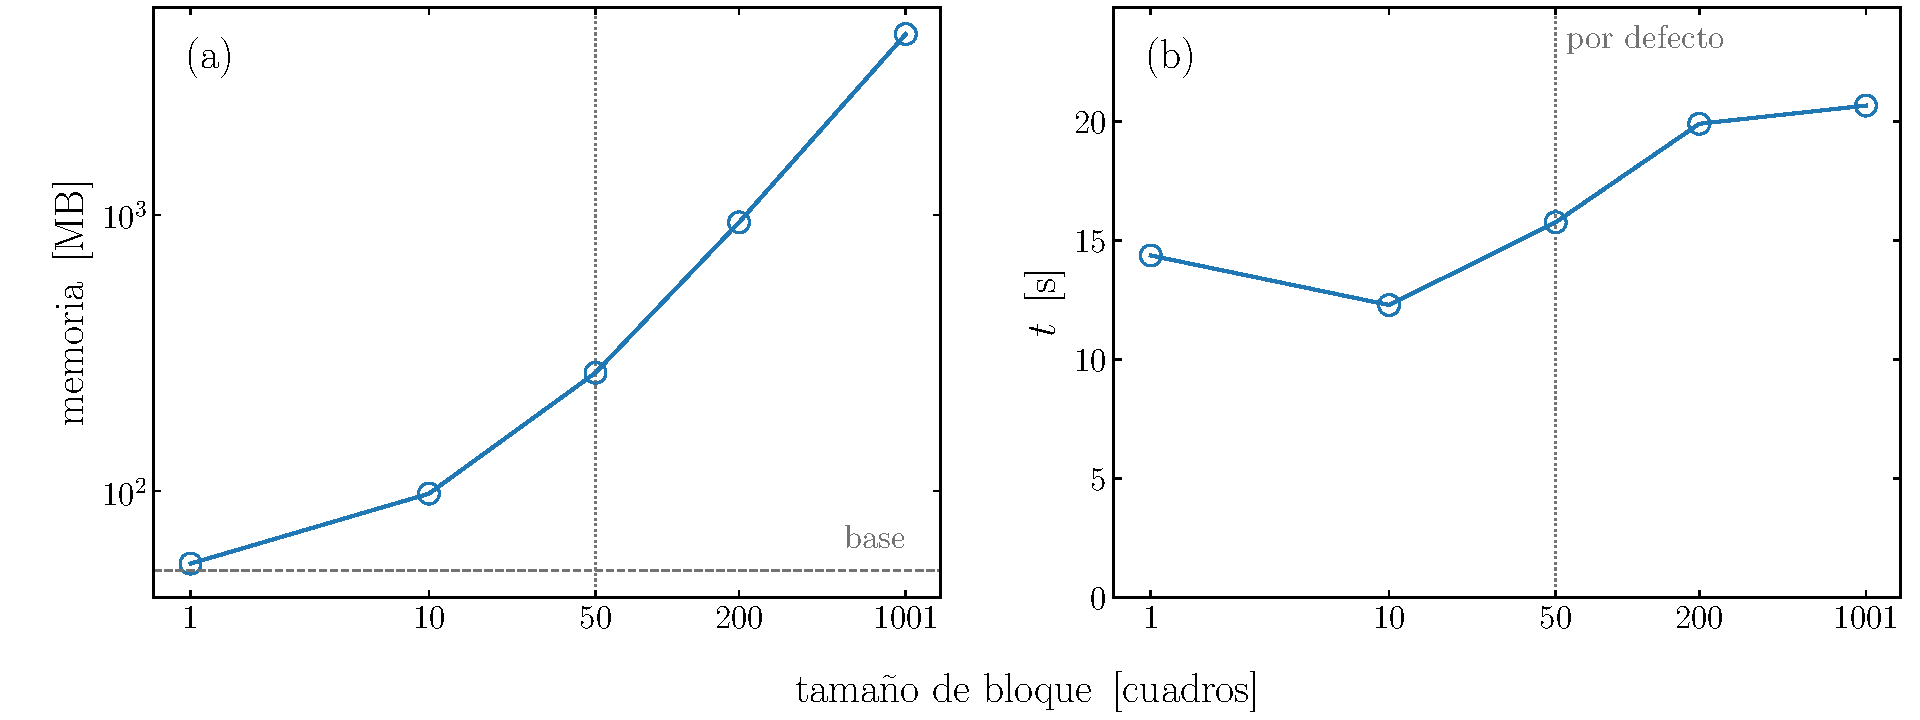
\includegraphics[width=\textwidth]{figuras/rendimiento.pdf}
\caption{Pico de memoria (a) y tiempo real (b) del análisis de una
trayectoria de \num{1001} cuadros según el tamaño de bloque; el tamaño
\num{1001} corresponde a la trayectoria entera en un solo bloque. La línea de
trazos marca la memoria base (intérprete, bibliotecas y metadatos), y la
punteada, el tamaño de bloque por defecto.}
\label{fig:rendimiento}
\end{figure}

La memoria crece linealmente con el tamaño de bloque, a razón de unos
\SI{4.5}{\mega\byte} por cuadro, desde \SI{55}{\mega\byte} con un cuadro por
bloque, apenas por encima de los \SI{51.5}{\mega\byte} de base, hasta
\SI{4.5}{\giga\byte} con la trayectoria entera en un solo bloque, que
equivale a cargarla completa, aunque sólo con las variables que los cálculos
usan. Con el
tamaño por defecto, de 50 cuadros, el pico es de \SI{268}{\mega\byte},
diecisiete veces menor, y no depende del largo de la trayectoria. El tiempo,
por su parte, no empeora al trabajar por bloques sino que mejora: el mínimo,
de \SI{12.3}{\second}, se alcanza con bloques de 10 cuadros, un 40\,\% menos
que con la trayectoria entera (\SI{20.7}{\second}), probablemente
porque los arreglos de un bloque chico aprovechan mejor la memoria caché del
procesador. Sólo con bloques de un cuadro el costo fijo de cada lectura
vuelve a hacerse notar.

Una ejecución del comando \comando{} con esos mismos cálculos sobre la misma
trayectoria, ya presente en la memoria caché del sistema operativo, tardó
\SI{16.5}{\second} con un pico de \SI{275}{\mega\byte}. Leída desde el disco
en red de un clúster, una trayectoria del mismo sistema llevó
\SI{62}{\second}, de los cuales sólo \SI{15}{\second} fueron de cálculo: en
ese caso el tiempo lo domina la lectura, y la lectura perezosa contribuye a
reducirlo, porque de los \SI{6}{\giga\byte} del archivo se leyeron sólo los
\SI{2.6}{\giga\byte} de las variables que los cálculos usan.

\subsection{Ejemplo de resultado}

La figura~\ref{fig:perfil} muestra el perfil de velocidad axial publicado
en~\cite{mosca2025}, como ejemplo del tipo de resultado que produce el
análisis. Se obtuvo con las herramientas originales; \paquete{} implementa
el mismo cálculo como \texttt{perfil-velocidad}, y su equivalencia con la
versión original está verificada en la tabla~\ref{tab:validacion}.

\begin{figure}[tb]
\centering
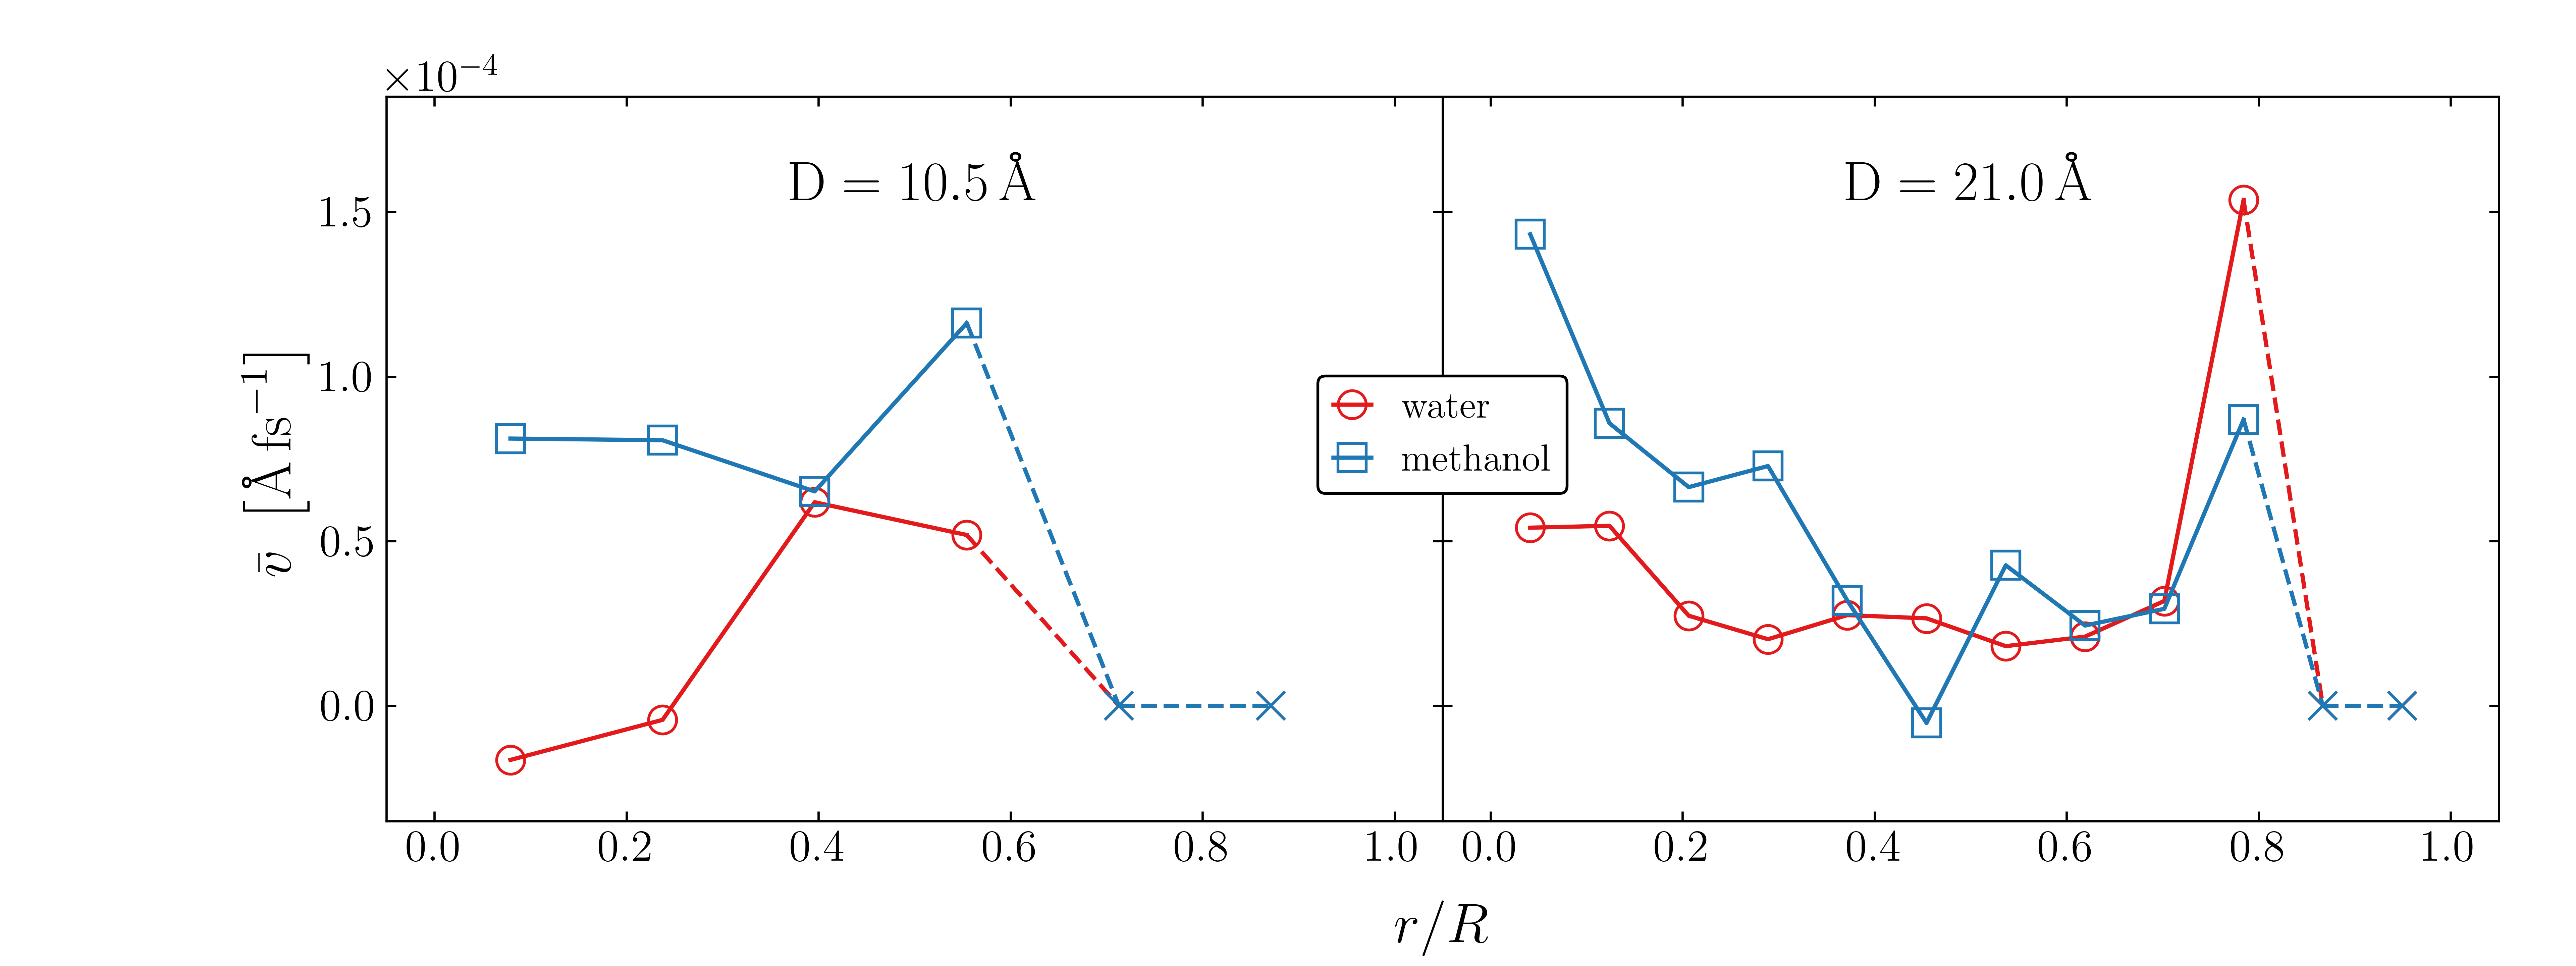
\includegraphics[width=\textwidth, trim=2.5cm 0 0 0, clip]{figuras/perfil_velocidad_articulo.png}
%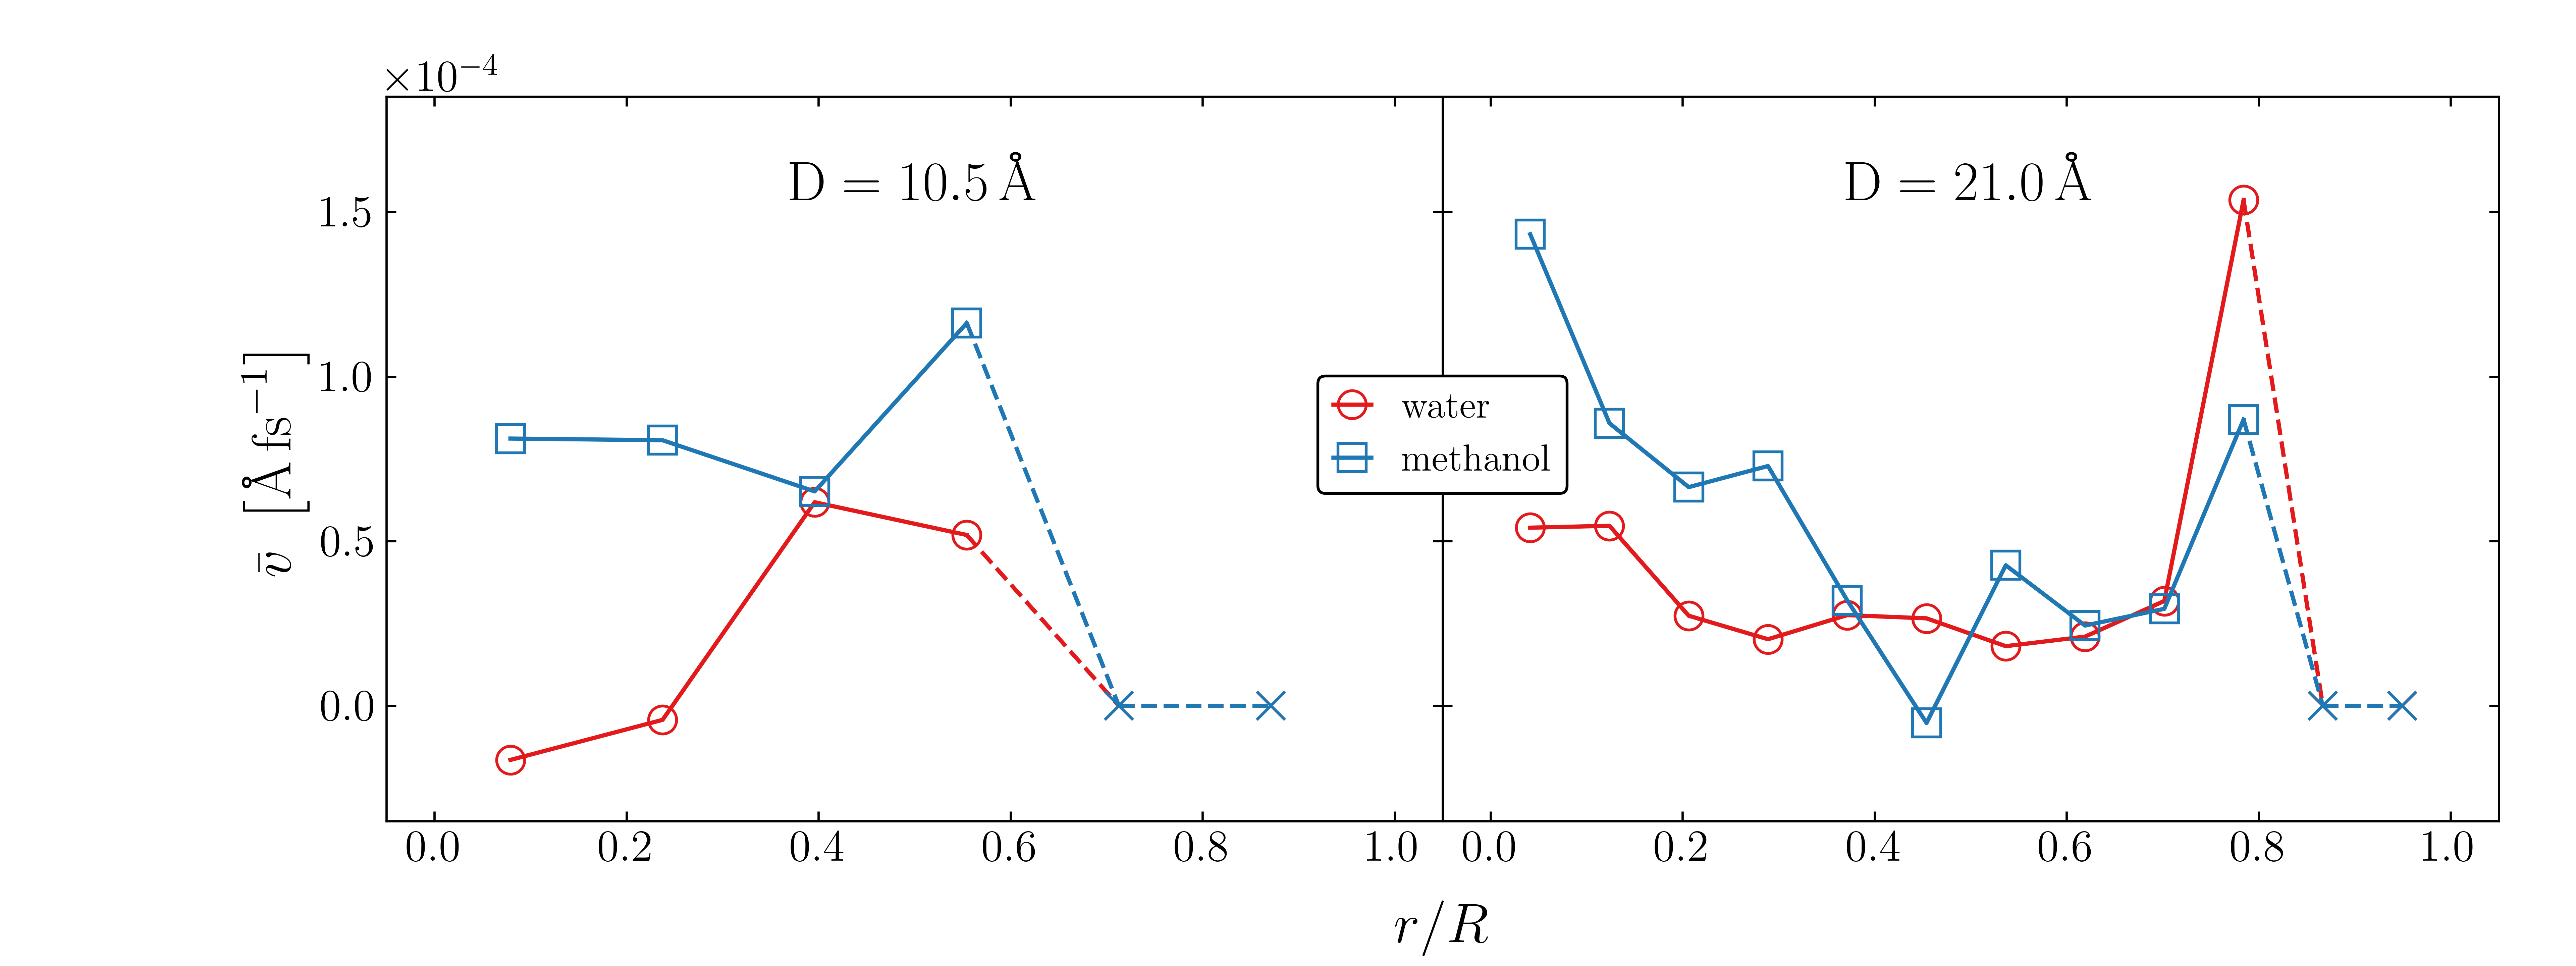
\includegraphics[width=\textwidth]{figuras/perfil_velocidad_articulo.png}
\caption{Perfil de velocidad axial de agua (\textit{water}) y metanol
(\textit{methanol}) en función de la distancia al eje, normalizada por el
radio del tubo, para la mezcla diluida durante la pervaporación, en los tubos
de \SI{10.5}{\angstrom} (izquierda) y \SI{21}{\angstrom} (derecha) de
diámetro. Las cruces indican los bins en los que no se contaron partículas.
Reproducida de~\cite{mosca2025}, donde se obtuvo con las herramientas de
análisis originales.}
\label{fig:perfil}
\end{figure}

%/ ======================================================================
\section{Conclusiones y trabajo futuro}

Los scripts de análisis con los que se obtuvieron los resultados
de~\cite{mosca2025} quedaron reescritos como \paquete, un paquete de Python
orientado a objetos, versionado en un repositorio público, instalable con
\texttt{pip} y documentado, que reproduce los resultados del código original
y de LAMMPS y que cualquier integrante del grupo puede instalar y usar desde
la línea de comandos o como biblioteca. La lectura por bloques hace que la
memoria necesaria dependa del tamaño de bloque y no del largo de la
trayectoria, con un pico diecisiete veces menor que el de cargarla completa y
sin pérdida de velocidad, y el marco de referencia del tubo elimina las
rotaciones, que eran la causa de que el análisis de los sistemas más grandes
agotara la memoria. Como trabajo futuro quedan incorporar las partes del código
original que no se reescribieron porque no forman parte del análisis de resultados:
las transformaciones de trayectorias y configuraciones (rotaciones, imágenes
periódicas, cambios de la longitud de la celda), propias de la preparación de
las simulaciones; el diagnóstico de la densidad de los reservorios, que se
usaba durante el llenado del tubo; y el cálculo del desplazamiento cuadrático
medio, que quedó fuera de los resultados publicados, y evaluar si conviene reducir
el tamaño de bloque por defecto a 10 cuadros, a la luz de las mediciones de rendimiento.

\printbibliography[heading=bibintoc, title={Referencias}]

\end{document}
